\tikzstyle{input_neuron}=[circle,draw=red!50,fill=red!10,thick,minimum size=4mm]
\tikzstyle{hidden_neuron}=[circle,draw=blue!50,fill=cyan!10,thick,minimum size=4mm]
\tikzstyle{output_neuron}=[circle,draw=green!50,fill=green!10,thick,minimum size=4mm]
\tikzstyle{cpy_neuron}=[circle,draw=red!50,fill=red!50,thick,minimum size=4mm]
\tikzstyle{input}=[circle,draw=black!50,fill=black!20,thick,minimum size=4mm]

\begin{tikzpicture}[scale=0.5, transform shape]
	
	\onslide<1->{
		\node [text width = 30mm] at (2.5,3){Region proposals};
		\node[inner sep=0pt] (A) at (2.5,1.8)
		{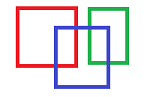
\includegraphics[scale = 0.9]{images/bboxes.png}};

		\node [text width = 34mm] at (6.5,3){Feature extraction};
		\node[inner sep=0pt] (A) at (6.5,2)
		{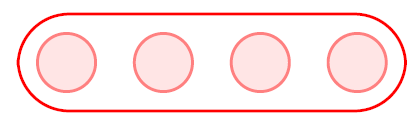
\includegraphics[scale = 0.5]{images/feature.PNG}};
		
		\node [text width = 25mm] at (11.5,3){Classifier};
		\node[inner sep=0pt] (A) at (11.0,2)
		{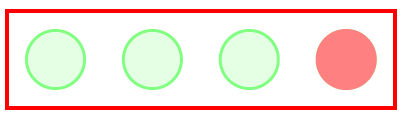
\includegraphics[scale = 0.5]{images/classification.PNG}};
	}
	
	\onslide<1->{
		\node [text width = 25mm] at (0,0){Pre 2012};
		\node[inner sep=0pt] (A) at (2.5,0.2)
		{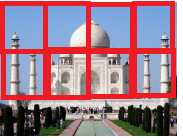
\includegraphics[scale = 0.6]{images/pre_2012.png}};
		\node[inner sep=0pt] (B) at (5.9,0.2)
		{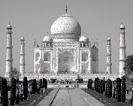
\includegraphics[scale = 0.8]{images/sift.PNG}};
		\node[inner sep=0pt] (C) at (8,0.2)
		{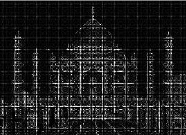
\includegraphics[scale = 0.6]{images/hog.PNG}};
		\node[inner sep=0pt] (D) at (11,0.4)
		{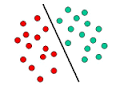
\includegraphics[scale = 0.45]{images/svm.PNG}};
	}
	

	\onslide<1->{
		\node [text width = 25mm] at (0,-1.5){RCNN};
		\node[inner sep=0pt] (A) at (2.5,-1.3)
		{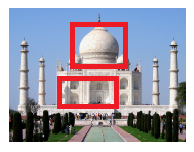
\includegraphics[scale = 0.6]{images/rcnn_bbox.png}};
		\node[inner sep=0pt] (B) at (6.8,-1.4)
		{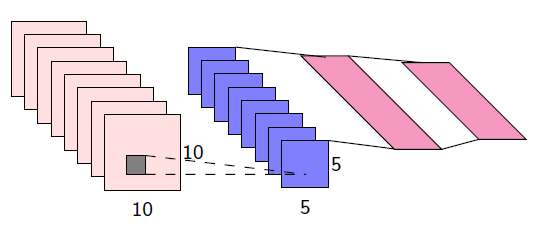
\includegraphics[scale = 0.4]{images/cnn.PNG}};
		\node[inner sep=0pt] (D) at (11,-1.2)
		{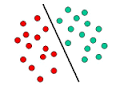
\includegraphics[scale = 0.45]{images/svm.PNG}};
	}
	
	\onslide<1->{
		\node [text width = 25mm] at (0,-3){
		Fast RCNN};
		\onslide<1->{\node[inner sep=0pt] (A) at (2.5,-2.8)
			{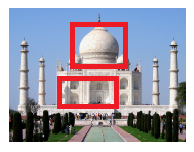
\includegraphics[scale = 0.6]{images/rcnn_bbox.png}};}
		\onslide<2->{\node[inner sep=0pt] (B) at (8.8,-2.9)
			{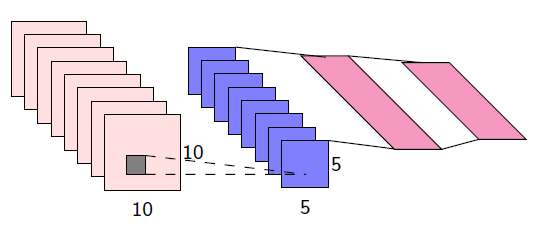
\includegraphics[height=1.5cm,width=6cm]{images/cnn.PNG}};}
		%\onslide<3->{\node[inner sep=0pt] (D) at (11,-2.8)
		%	{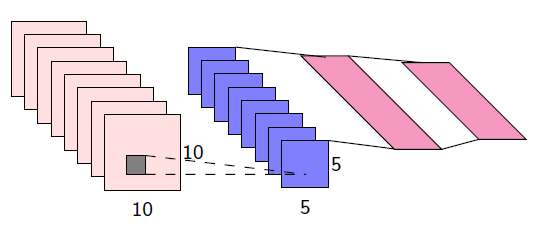
\includegraphics[scale = 0.4]{images/cnn.PNG}};}
	}
	
\end{tikzpicture}
